\newcommand{\secorio}{\href{https://www.secorio.com/}{
\includegraphics[width=2cm]{images/logo_comodo.png}\tiny via Secorio}}

\subsection{Get an S/MIME certificate}\label{catable}
You have a choice in whether you want to subscribe to a Certificate
Authority (``CA'') or whether you want to be your own CA and generate
your keys manually.  The advantage of using a CA is that the recipient
has less key management effort (this doesn't matter if Justin is your
recipient).  But CA subscriptions cost money in some situations and
also limit the validity period of the key.

\textbf{If you want to create your own key} using Windows, install
\href{https://slproweb.com/products/Win32OpenSSL.html}{OpenSSL for
  Windows}.  Mac users will already have openssl installed.  Then
follow
``\href{https://www.howtoforge.com/how-to-encrypt-mails-with-ssl-certificates-s-mime#-alternative-create-a-certificate-authority-to-sign-a-certificate}{%
  Create a Certificate Authority to Sign A Certificate}'' to create
your own CA and personal key pairs.

\textbf{If you're opting to use a CA}, then browse to one of these
certificate authorities (Justin recommends Comodo via Secorio):\\

\rowcolors{2}{Khaki}{LightGoldenrodYellow} %this breaks old versions of dvisvgm!
\begin{tabular}{m{38mm}p{2.3cm}l>{\tiny}p{0.36\textwidth}}
  \slshape\textbf{CA}
  & \slshape\textbf{price} \newline\tiny(for non-commercial individual use)
  & \slshape\textbf{validity}
  & \slshape\normalsize\textbf{notes}\\
  %\hline\\
  \href{https://www.cacert.org/}{
\includegraphics[width=2cm]{images/logo_cacert4.png}} & gratis & 6|24 mos.\tiny (\href{http://wiki.cacert.org/FAQ/Privileges}{criteria}) & community driven; getting a 2yr cert requires meeting w/someone and showing state-issued proof of id\\
  \href{https://secure.comodo.com/products/frontpage?area=SecureEmailCertificate}{
\includegraphics[width=2cm]{images/logo_comodo.png}\tiny direct} & gratis & 1 yr &\\
  \href{https://www.instantssl.com/ssl-certificate-products/free-email-certificate.html}{
\includegraphics[width=2cm]{images/logo_comodo.png}\tiny via InstantSSL} & gratis & 1 yr &\\
  \secorio & gratis & 1 yr & simple; assumed choice by this guide\\
  \href{https://www.entrust.com/secure-email-certificates/}{
\includegraphics[width=2cm]{images/logo_entrust.png}} & $\geq$\$20 & &\\
  \href{https://www.identrust.com/certificates/trustid.html}{
\includegraphics[width=2cm]{images/logo_trustid.png}} & $\geq$\$19 & &\\
  \href{https://www.startcomca.com/}{
\includegraphics[width=2cm]{images/logo_startcom.png}} & gratis & 2 yrs & distrusted by Mozilla and others, thus signed msgs will likely be seen as invalid unless recipients manually add Startcom's CA key to their keystore\\
  \href{https://buy.wosign.com/free/}{\begin{overpic}[width=2cm]{images/logo_wosign.png}\put(-5,10){\color{black}\rule{24mm}{1pt}}\end{overpic}} & \st{gratis} n/a & \st{2 yrs} n/a & recently \textbf{discontinued} but still maintained in this list because they intend to return to business\\
\end{tabular}\\

% geotrust, symantec, thawte have discontinued service
% (the "\par" at the end of this ensures that the linespacing is sensible)
{\tiny Warning: the CAs that participate in e-mail certificate
  verification are constantly changing.  Many CAs have discontinued
  e-mail certification prior to this guide.  Those with no intent to
  return to service are omitted here, but some of the above listings
  are likely to become obsolete as this guide ages.  Consequently it
  might be interesting to check out the catalog of certificate
  authorities listed at
  \url{http://kb.mozillazine.org/Getting_an_SMIME_certificate}).\par}

\begin{minipage}{\textwidth}
\subsubsection{If you chose ``Comodo via Secorio''}
\begin{multicols}{2}
  \begin{enumerate}
  \item (secorio.com) If you are using the \emph{noscript} firefox
    plugin, you must enable javascript for \texttt{secorio.com} and
    \texttt{comodo.com}.
  \item (secorio.com) In the left frame, select ``\texttt{S/MIME Class
      2}'' (even though it's \emph{class 1} that we need), then click
    ``\texttt{Order}''.
  \item (secorio.com) Scroll down to ``\texttt{S/MIME Certificates}''
    and choose ``1 year'' in the pull-down to the right of the
    \emph{class 1} row.
  \item (comodo.com) Fill out the form that appears in a new tab.
    Setting a revocation password is optional (and it's a good
    idea).% Untick the
    % ``Comodo newsletter opt in'' crap (if it's there).
  \item (your inbox) An e-mail will arrive.  If your e-mail client
    renders it graphically, click the button ``\texttt{Click \&
      Install Comodo Email Certificate}''.  For text clients, follow
    the instructions in the e-mail.  If your mail client does not
    automatically use Firefox or IE to open URLs, right-click that
    button instead, copy the URL, and paste it in the address bar to
    force it to render in Firefox or IE.
  \item Skip to section~\ref{cert_install}
  \end{enumerate}
\end{multicols}
\end{minipage}\\[1em]
  
\begin{minipage}{\textwidth}
  \subsubsection{If you chose ``StartCom''}
  \begin{multicols}{2}
    \begin{enumerate}
    \item (startcomca.com) 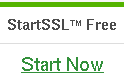
\includegraphics[width=0.1\textwidth]{images/startcomca_step1}
    \item (startcomca.com) 
\includegraphics[width=0.1\textwidth]{images/startcomca_step2_signup}
    \item (startcomca.com) Fill out the form.
    \item (your e-mail account) A verification code will arrive.
    \item (startcomca.com) Enter the verification code, click ``sign up''.
      
      The system could not install the login certificate
      automatically, you should install it manually.  Create a
      ``Private key password'' Please click here to install the
      issuing CA certificate into your browser first.  save a *.p7b
      file
      
    \item Skip to section~\ref{cert_install}
    \end{enumerate}
  \end{multicols}
\end{minipage}

\subsubsection{If you chose another certificate authority}
Simply follow the instructions on the website of the CA.  It will
generally involve filling out a form and confirming an e-mail.
